\begin{tikzpicture}[remember picture, scale=\modDGHyperScale]
% dummy
\coordinate[overlay] (\modIdPrefix v-coord-0-0) at (0.78567, 1.5207) {};
\coordinate[overlay] (\modIdPrefix v-coord-1-0) at (3.5746, 1.0129) {};
\coordinate[overlay] (\modIdPrefix v-coord-2-0) at (2.0032, 0.25) {};
\coordinate[overlay] (\modIdPrefix v-coord-3-0) at (1.6309, 3.0659) {};
\coordinate[overlay] (\modIdPrefix v-coord-4-0) at (3.3475, 2.7365) {};
\coordinate[overlay] (\modIdPrefix v-coord-5-0) at (2.2607, 1.7168) {};

% id = 0, graphName = g_{0}
\node[modStyleDGHyperVertex, at=(v-coord-0-0)] (v-0-0) {\includegraphics[scale=\modDGHyperImageScale] {\modInputPrefix/out/002_g_0_11311100.pdf}\\{$\mathrm{g_{0}}$}};
% id = 1, graphName = g_{1}
\node[modStyleDGHyperVertex, at=(v-coord-1-0)] (v-1-0) {\includegraphics[scale=\modDGHyperImageScale] {\modInputPrefix/out/004_g_1_11311100.pdf}\\{$\mathrm{g_{1}}$}};
% id = 2, graphName = p_{0,0}
\node[modStyleDGHyperVertex, at=(v-coord-2-0)] (v-2-0) {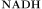
\includegraphics[scale=\modDGHyperImageScale] {\modInputPrefix/out/006_g_2_11311100.pdf}\\{$\mathrm{p_{0,0}}$}};
% id = 3, graphName = p_{0,1}
\node[modStyleDGHyperVertex, at=(v-coord-3-0)] (v-3-0) {\includegraphics[scale=\modDGHyperImageScale] {\modInputPrefix/out/008_g_3_11311100.pdf}\\{$\mathrm{p_{0,1}}$}};
% id = 4, graphName = p_{0,2}
\node[modStyleDGHyperVertex, at=(v-coord-4-0)] (v-4-0) {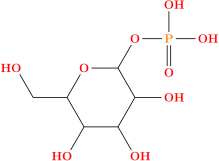
\includegraphics[scale=\modDGHyperImageScale] {\modInputPrefix/out/010_g_4_11311100.pdf}\\{$\mathrm{p_{0,2}}$}};
% id = 5{ 'g_{0}' 'g_{1}' }, 'R1: (S)-lactate + NAD+ = pyruvate + NADH + H+', { 'p_{0,0}' 'p_{0,1}' 'p_{0,2}' }
\node[modStyleDGHyperEdge, at=(v-coord-5-0)] (v-5-0) {$\mathrm{r_{0}}$};
% id = 5{ 'g_{0}' 'g_{1}' }, 'R1: (S)-lactate + NAD+ = pyruvate + NADH + H+', { 'p_{0,0}' 'p_{0,1}' 'p_{0,2}' }
\path[modStyleDGHyperConnector] (v-0-0) to (v-5-0);
\path[modStyleDGHyperConnector] (v-1-0) to (v-5-0);
\path[modStyleDGHyperConnector] (v-5-0) to (v-2-0);
\path[modStyleDGHyperConnector] (v-5-0) to (v-3-0);
\path[modStyleDGHyperConnector] (v-5-0) to (v-4-0);
\end{tikzpicture}%
